\chapter{Instalación del sistema en la SmartFridge}
En esta sección se va a explicar como se instala y configura todo el sistema en el frigorífico, además de la impresión de piezas necesarias para la instalación de éste.

Hay que instalar un sensor RFID, un sensor de nivel de agua, dos sensores magnéticos y sus receptores, y doce sensores de peso. Además de cinco controladores que administren estos sensores.

\section{Impresión 3D}
Para hacer la instalación de los sensores y controladores, se necesita una estructura para guardar los controladores o insertar los sensores para dejarlos acoplados en una posición del frigorífico. Como éste no está preparado para esta implementación, se tienen que crear modelos 3D con las piezas necesarias para conseguir que los sensores se acoplen al frigorífico y funcionen correctamente.

\subsection{Software utilizado}
El software utilizado ha sido dos:

\begin{itemize}
    \item \textbf{Tinkercad}
    \item \textbf{Ultimaker Cura}
\end{itemize}

Ambos software son explicados en la sección de herramientas de desarrollo (Sección 1.3.3) Con el primer software se van a crear los modelos que se necesitan para imprimir. Con el segundo, se elige la impresora a usar, se configura el tipo de plástico, se introduce el modelo, se segmenta y se imprime.

\subsection{Modelos 3D}
Para el sensor RFID se debe usar un recipiente para guardar el propio sensor, el controlador, la batería y los LEDs que dan información. Para ello se ha hecho una caja con dos compartimentos a medida para poder guardar todos estos componentes, un hueco para dejar el sensor RFID y unos huecos para introducir los LEDs y que sean vistos por el usuario (ver Figura \ref{fig:rfidmodel}).

Para el sensor del nivel de agua, sensores magnéticos y sensor de peso del cajón del embutido, que van conectados a un mismo controlador, se necesitan dos modelos 3D. Uno para guardar el controlador y la batería (ver Figura \ref{fig:controllermodel}) y también un modelo para poner los pesos como patas de una superficie que irá en el cajón del embutido (ver Figura \ref{fig:weightmodel}). Los sensores magnéticos y el del nivel de agua no necesitan modelos 3D para ser instalados.

Para los sensores de peso que se instalan en los basares de la puerta y que van conectados a un tercer controlador, se necesitaría un modelo para el controlador y la batería (ver Figura \ref{fig:controllermodel}) y una superficie para poner los sensores de peso como en la Figura \ref{fig:weightmodel}, pero de diferente tamaño.

Para el cuarto y quinto controlador, se van a utilizar mas sensores de peso y van al cajón de fruta y verduras. El cajón del frigorífico es muy grande, por lo que se va a dividir el cajón en dos cajones más pequeños. Por ello hay que hacer dos modelos 3D que al juntarlos creen dos cajones. El cajón izquierdo (ver Figura \ref{fig:leftmodel}) está formado por una superficie donde tiene los soportes para los sensores de peso, y una pared lateral y trasera. No necesita más porque el cajón se completa con las paredes el cajón del frigorífico. El cajón derecho (ver Figura \ref{fig:rightmodel}) solo necesita una superficie con una pared trasera. Si se imprime esto y se introduce en el cajón grande del frigorífico, se conseguirá dividirlo en dos más pequeños.

Detrás de los modelos 3D, se queda un pequeño hueco entre el cajón del frigorífico y los creados con los modelos 3D. Ese espacio se utilizará para guardar el controlador y las baterías con el modelo de la Figura \ref{fig:controllermodel}. Cada modelos de imprimirá con una medida diferente para adaptarse al hueco del frigorífico donde hay que hacer la instalación de los modelos impresos.

\begin{figure}[h]
 \centering
  \subfloat[Sensor RFID]{
   \label{fig:rfidmodel}
    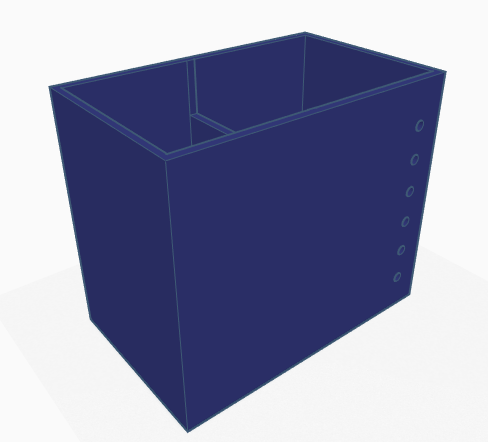
\includegraphics[width=.40\textwidth]{capitulos/capitulo9/RFID.png}}
  \subfloat[Controlador y batería.]{
   \label{fig:controllermodel}
    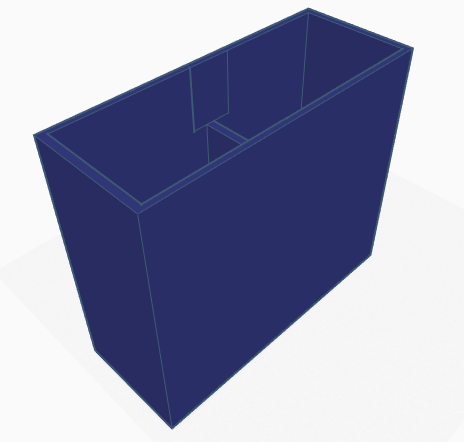
\includegraphics[width=.38\textwidth]{capitulos/capitulo9/controladorYBateria.png}}
 \caption{Modelos 3D.}
\end{figure}

\begin{figure}[h] 
    \centering
    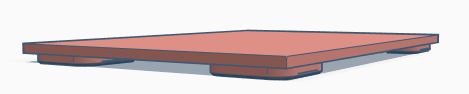
\includegraphics[width=.70\textwidth]{capitulos/capitulo9/peso.png}
    \caption{Modelo 3D - Peso.}
    \label{fig:weightmodel}
\end{figure}

\begin{figure}[h]
 \centering
  \subfloat[Cajón izquierdo.]{
   \label{fig:leftmodel}
    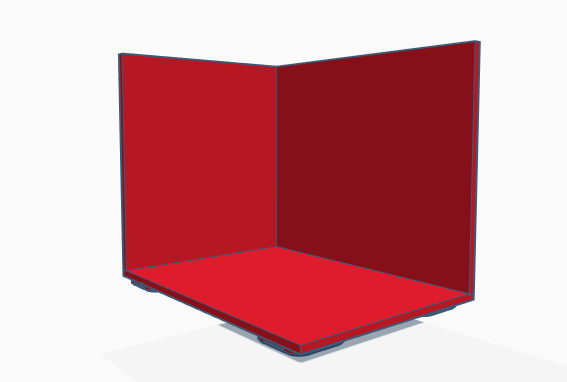
\includegraphics[width=.40\textwidth]{capitulos/capitulo9/cajonIzquierdo.png}}
  \subfloat[Cajón derecho.]{
   \label{fig:rightmodel}
    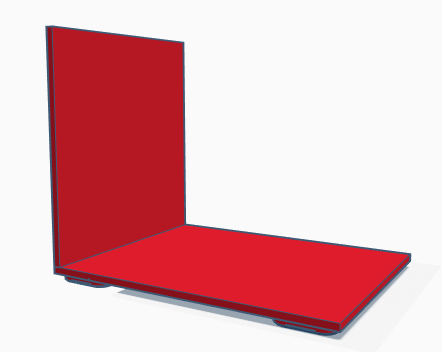
\includegraphics[width=.40\textwidth]{capitulos/capitulo9/cajonDerecho.png}}
 \caption{Modelos 3D.}
\end{figure}

\section{Impresión del modelo}
Una vez que se tienen los modelos 3D necesarios para imprimir, se debe de usar el programa “Ultimaker Cura” para configurar la impresora de impresión, el material, el modelo y segmentarlo e imprimirlos.

Para este proyecto se va a usar la impresora “Prusa i3 MK3S” y de material “PLA”, por lo que se configura estos parámetros en el programa (Figura \ref{fig:prusa}).

\begin{figure}[h] 
    \centering
    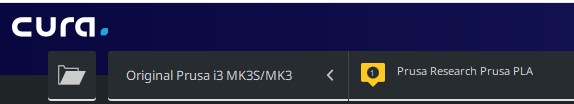
\includegraphics[width=.50\textwidth]{capitulos/capitulo9/prusa.png}
    \caption{Configuración de Ultimaker Cura.}
    \label{fig:prusa}
\end{figure}

A continuación, se carga el modelo 3D en el programa y se segmenta. Al segmentarlo (Figura \ref{fig:segmentation}) se puede ver diferente información, como el número de capas que va a tener (1333), el tiempo que va a tardar en hacer la pieza (1 día y 1h) o hasta la cantidad de gramos que va a gastar de PLA (253g).

\begin{figure}[h] 
    \centering
    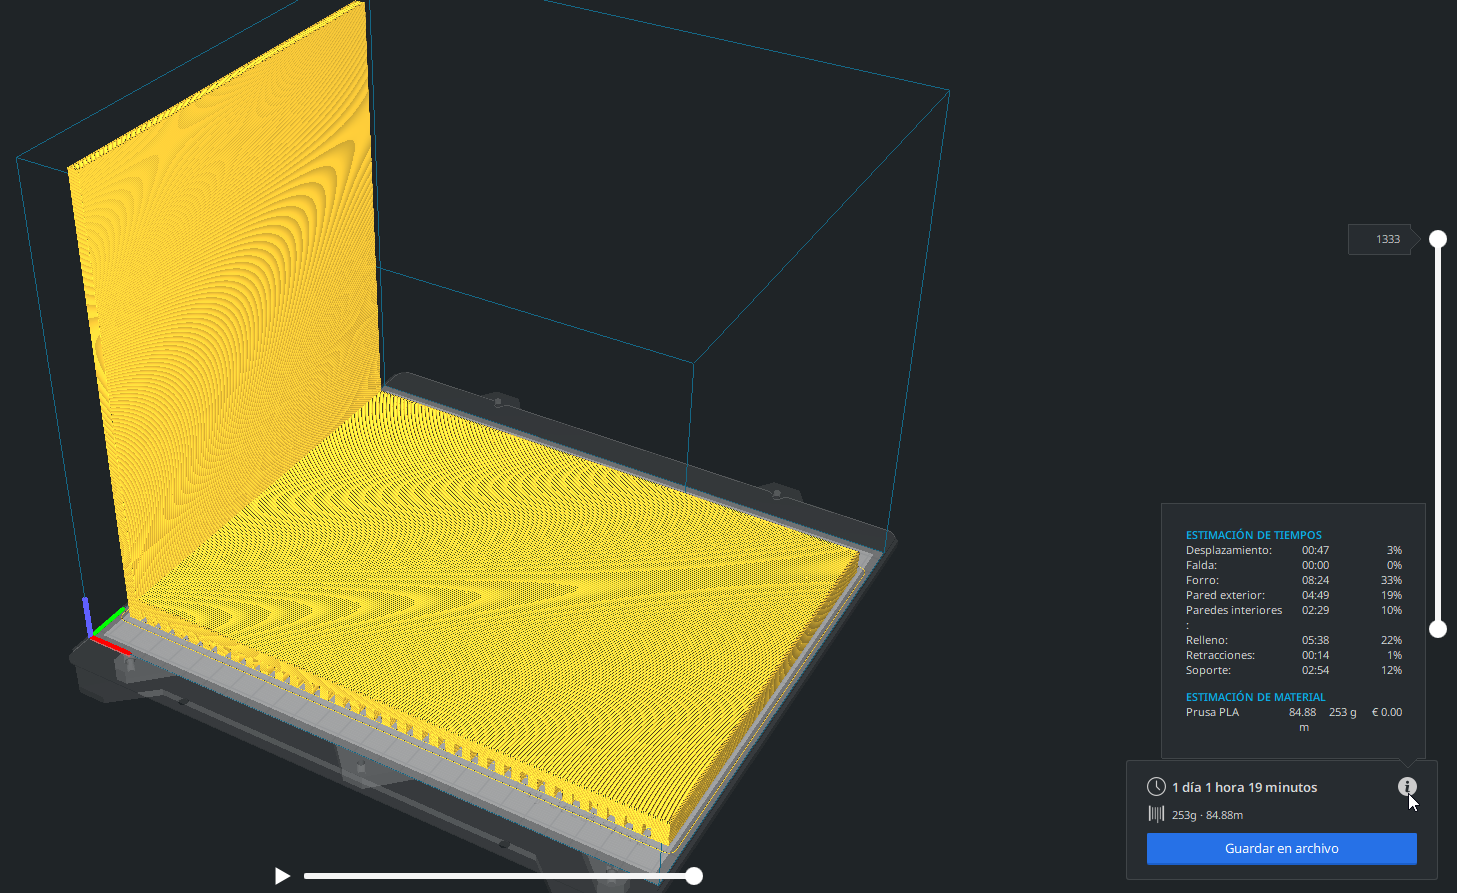
\includegraphics[width=.90\textwidth]{capitulos/capitulo9/segmentation.png}
    \caption{Segmentación del modelo 3D.}
    \label{fig:segmentation}
\end{figure}

Finalmente, se puede guardar el archivo segmentado, cargarlo en la impresora e imprimirlo.

\section{Proceso de instalación}
En el proceso de instalación se va a explicar como instalar todo el sistema, desde los sensores, pasando por los controladores y el sistema.

Los sensores y controladores se deben de colocar de la siguiente manera:

\begin{itemize}
    \item \textbf{Primer controlador:} Se debe de colocar fuera del frigorífico, con su sensor RFID y su batería dentro del recipiente impreso.
    \item \textbf{Sensor magnético:}  Se coloca en las dos puertas que tiene el frigorífico, en la parte exterior.
    \item \textbf{Sensor de nivel de agua:} Se coloca en el recipiente de agua del frigorífico, por la parte exterior y a la altura que se considere que es necesario avisar para rellenar el depósito.
    \item \textbf{Segundo controlador:} Se coloca en el interior del frigorífico, en el cajón del embutido cubierto por su recipiente impreso. En este controlador va conectado el peso del cajón de embutidos, que también estará adaptado con su pieza impresa, los dos receptores de los sensores magnéticos y el sensor de nivel de agua.
    \item \textbf{Tercer controlador:} Va colocado en uno de los basares de la puerta del frigorífico, cubierto con su recipiente impreso. En éste van conectados seis sensores de peso repartidos por los diferentes basares de la puerta, donde se diferenciará entre huevos, refrescos y briks de leche. Cada peso lleva también su adaptación impresa para su correcto funcionamiento.
    \item \textbf{Cuarto y quinto controlador:} Ambos controladores van a funcionar igual, solamente que uno es para el cajón de las verduras y el otro es para el cajón de las frutas. En estos cajones va a ir un controlador en su recipiente impreso, y dos pesos con una estructura impresa que divide cada cajón en dos cajones más pequeños.
\end{itemize}

Se puede apreciar una representación gráfica de la instalación de los sensores en la Figura \ref{fig:sensoreslg} y de los controladores en la Figura \ref{fig:controllerlg}.

El sistema está configurado para encenderse y ejecutarse todo automáticamente, por lo que simplemente conectándolo a la red de alimentación y a la red donde estén conectados los controladores, sería suficiente para que todo se ejecutara automáticamente. El sistema puede alojarse dónde sea más conveniente, siempre y cuando esté conectado a la misma red que los controladores.